\pdfoutput=1

\documentclass[11pt]{article}

\usepackage{graphicx}

\usepackage[]{acl}
\usepackage{tabularx}

\usepackage{times}
\usepackage{latexsym}

\usepackage[T1]{fontenc}
\usepackage[utf8]{inputenc}

\usepackage{microtype}

\title{Examining readability of text generated through GPT-3 }

\author{Aron Winkler \\
  University of Tübungen \\
  \texttt{winkler.aron5@gmail.com}}

\begin{document}
\maketitle
\begin{abstract}
    This paper examines readability-related metrics of AI-generated text, specifically texts produced by OpenAI's GPT-3. Generation was performed across 10 topics and the 6 proficiency levels defined by the CEFR framework, and outputs were compared with Simple Wikipedia and (standard) Wikipedia articles on the same topics.
\end{abstract}

\section{Introduction}

AI text generation has experiences a massive rise in popularity with the media reach achieved by the release of OpenAI's GPT-3 \citep{brown2020language} and its chat GUI interface ChatGPT\footnote{\url{https://openai.com/blog/chatgpt}}. While early public opinion focused on how - in the school setting - it would be students who would benefit from the new system by having their schoolwork done for them, little was said about how AI text generation could become an asset for didactitians in generating teaching material.

AI text generation might become an important tool for teachers, allowing them to generate learning material about topics and events that engage their students that might not be available on the market. An interesting setting for such a phenomenon is language learning, where it is necessary to produce learning material for students at different proficiency levels: whether to create ex-novo or simplify existing text material, AI text-generation tools can easily be imagined as having an enabling effect. 

It is however not obvious that AI generation tools reach the desired quality or adherence to the didactic goals that teachers set out. Owing to the increased popularity of these tools, more research is desirable on their applicability in a number of different settings.

This work aims to make a contribution to those questions by verifying the readability level of text content generated by GPT-3 with regard to 10 topics and the 6 proficiency levels defined by the CEFR framework. A number of complexity metrics are computed on the generated texts and compared with Simple Wikipedia\footnote{\url{https://simple.wikipedia.org/wiki/Main_Page}} as well as Wikipedia\footnote{\url{https://www.wikipedia.org/}} articles on the same topics in order to gauge the true readability levels of the model outputs.
\section{Dataset and metrics}
\subsection{Dataset}

OpenAI's REST api was employed to produce texts with the "text-davinci-003" model (a GPT-3 variant) across 10 topics\footnote{'Color Blindness, The Great Depression, Butterflies, Dogs, Semantics, The Internet, The Moon, Dinosaurs, Economics, Quantum Mechanics'} and 6 CEFR proficiency levels\footnote{A1, A2, B1, B2, C1, C2}. Topics were selected without any particular guiding principle other than a general goal of variety between events, entities, and phenomena. The prompts fed to the model followed the template:

\begin{quote}
  \emph{Write a text for learners of English at the [level] level about [topic].}
\end{quote}

In addition to the 60 texts obtained in this way, the dataset was enriched by Simple Wikipedia and Wikipedia articles corresponding to each of the 10 topics, resulting in an additional 20 dataset entries.

\subsection{Preprocessing}

Preprocessing of the dataset comprised enrichment with POS and dependency annotation. Part-of-speech tagging was achieved with nltk \citep{LoperBird02} and dependency relations were added through nltk in conjunction with CoreNLP models \citep{corenlp}.

\subsection{Metrics}

\begin{table}[ht]
    \centering
    \begin{tabular}{p{110px}c}
        \hline
        \textbf{Metric} & \textbf{Abbreviation} \\
        \hline
        Sentence length & ASL \\
        \hline
        Noun to verb ratio & NVR \\
        \hline
        Type Token Ratio (first 100 tokens) & TTR \\
        \hline
        Clauses Per Sentence & CPS \\
        \hline
        Length of Longest Dependency Link & LLDL \\
        \hline
        Parse Tree Depth & PTD \\
        \hline
        Ratio of words in top 3000 English words & WIT \\
        \hline
    \end{tabular}
    \caption{Readability metrics}
    \label{tab:metrics}
\end{table}

Table~\ref{tab:metrics} lists the readability metrics used in this experiment. This specific selection was inspired by \citep{venturi-etal-2015-nlp}, but many more examples of their usage can be found. 

This feature set almost exclusively targets lexis and syntax, with little regard for morphology outside of the noun-to-verb ratio feature. While this is a limitation of this set, the language of this experiment is solely English, a language not necessarily known for a complex morphological system.

The feautre "Words in Top 3000 English words" uses unigram frequencies from the Google Web Trillion Word corpus\footnote{\url{https://ai.googleblog.com/2006/08/all-our-n-gram-are-belong-to-you.html}} to isolate the 3000 most frequent words of the English language. Many research approaches to readability employ similar ideas to gain insight into the lexical complexity of texts, such as the BIV (basic Italian vocabulary) employed by \citep{dellorletta-etal-2011-read}.

All feature values outside of type-token-ratio (which ignores sentence boundaries) are computed at the sentence level. When a dataset entry comprises multiple sentences, the output for that entry is the average of the values for the sentences that compose it. 

\section{Results}

\begin{table*}[ht]
    \centering
    \begin{tabular}{lccccccc}
        \hline
        \textbf{Level} &       \textbf{ASL} &      \textbf{NVR} &      \textbf{TTR} &      \textbf{CPS} &      \textbf{LLDL} &      \textbf{PTD} &      \textbf{WIT} \\
        \hline
        S Wiki &  18.145            &  \textbf{1.918}   &  \textbf{0.661}   &  1.629            &   7.868           &  4.629            &  \textbf{0.749} \\
        \hline
        A1     &  18.539            &  1.681            &  0.657            &  1.932            &     8.0           &  5.113            &           0.83 \\
        \hline
        A2     &  20.717            &  1.477            &  0.648            &  \textbf{2.104}   &   8.843           &  5.415            &           0.828 \\
        \hline
        B1     &  19.124            &  1.607            &   0.65            &  \textbf{2.114}   &   8.416           &  5.383            &           0.826 \\
        \hline
        B2     &  20.766            &  1.694            &  0.632            &  \textbf{2.064}   &   \textbf{9.148}  &   5.64            &           0.821 \\
        \hline
        C1     &  \textbf{21.24}    &  \textbf{1.848}   &  0.646            &  1.967            &   9.147           &  \textbf{5.549}   &           0.804 \\
        \hline
        C2     &  \textbf{21.94}    &  1.836            &  \textbf{0.658}   &   1.94            &  \textbf{10.189}  &  \textbf{5.427}   &  \textbf{0.791} \\
        \hline
        Wiki   &  \textbf{26.131}   &  \textbf{2.342}   &  \textbf{0.667}   &  1.876            &  \textbf{11.323}  &  \textbf{5.681}   &  \textbf{0.678} \\
        \hline
    \end{tabular}
    \caption{
        \centering
        Average metric results for each difficulty level and metric. The 3 hightest values are highlighted for each metric. For WIT, the lowest 3 are highlighted instead.
    }
    \label{tab:means}
\end{table*}

Table~\ref{tab:means} details the average output for each difficulty level and metric. For each metric, the 3 values most indicative of low readability are highlighted.

With regards to the selected metrics, GPT-3 does a good job generating texts for the target readability level in the sense that prompts requesting C1 and C2 level material on average yield the least readable texts, whereas lower proficiency levels tend to have scores indicating higher readability.
 
While no rigorous checks are carried out in this paper in reference to the correlation between these metrics and article readability levels, it's still possible to examine some of the results to gain some insight into the black box that is GPT-3.

\begin{figure}[ht]
    \centering
    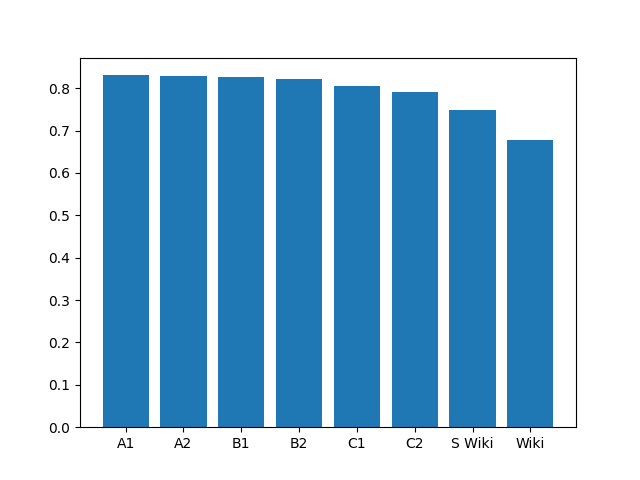
\includegraphics[width=\columnwidth]{figs/assets/plot-WIT.png}
    \caption{Mean metric values for WIT.}
    \label{fig:wit-mean}
\end{figure}

Among the selected measures, WIT (ratio of words in the 3000 most frequent English words) appears to be the most well-behaved, insofar as the prompted CEFR levels mostly maintain their natural progression. Figure~\ref{fig:wit-mean} shows the isolated scores for the WIT metric, which show a correlation with difficulty. Wikipedia and Simple Wikipedia articles have lower values, however this is possibly connected to those texts being several times longer.

\begin{figure}[h]
    \centering
    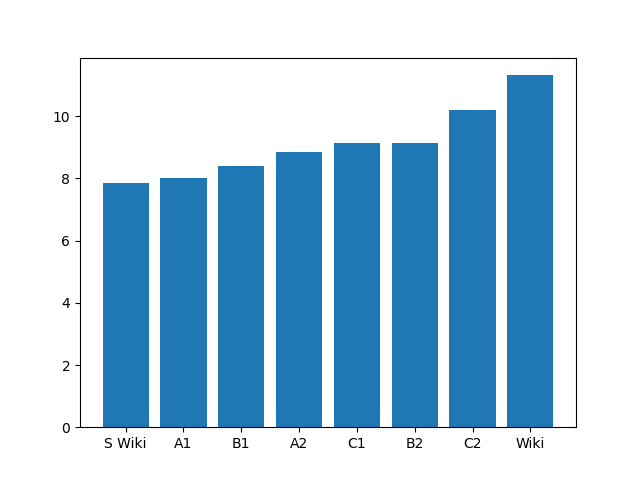
\includegraphics[width=\columnwidth]{figs/assets/plot-LLDL.png}
    \caption{Mean metric values for LLDL.}
    \label{fig:wit-mean}
\end{figure}

LLDL (length of longest dependency link) is another metric that performs well in terms of level differentiation. It also reflects the common belief that the biggest difficulty spike in language learning - as shown by Figure~\ref{fig:lldl-mean}. As with most metrics, however, the natural progression of the CEFR levels is lost, particularly in the middle portions.


\section{Discussion and future research}

This work attempted to gauge true readability levels of GPT-3 output texts with prompts across 10 topics and CEFR proficiency levels, optimising thus for the second language learning application environment. Outputs computed from the metrics set suggest that GPT-3 is at least somewhat aware of syntax and lexis when performin generation for a target readability level.

Future research into this topic could explore a wider variety of textual metrics, as this work only selected a handful that lent themselves particularly well to interpretation and did not require steep hardware requirements to obtain.

\section*{Acknowledgements}


\bibliography{anthology,custom}

\appendix
\section*{Resources}

\label{sec:appendix}

All code for this paper is available at \url{https://github.com/waron97/nlp_for_readability_term_paper}.

\end{document}